\documentclass[12pt, twoside]{article}
\usepackage[letterpaper, margin=1in, headsep=0.5in]{geometry}
\usepackage[english]{babel}
\usepackage[utf8]{inputenc}
\usepackage{amsmath}
\usepackage{amsfonts}
\usepackage{amssymb}
\usepackage{tikz}
\usetikzlibrary{quotes, angles}
\usepackage{graphicx}
\usepackage{enumitem}
\usepackage{multicol}

\newif\ifmeta
\metatrue %print standards and topics tags

\title{Regents Geometry}
\author{Chris Huson}
\date{September 2020}

\usepackage{fancyhdr}
\pagestyle{fancy}
\fancyhf{}
\renewcommand{\headrulewidth}{0pt} % disable the underline of the header
\raggedbottom


\fancyhead[LE]{\thepage}
\fancyhead[RO]{\thepage \\ Name: \hspace{4cm} \,\\}
\fancyhead[LO]{BECA / Dr. Huson / Geometry 02 Area and volume}

\begin{document}

\subsubsection*{2.2 CW Compound areas}
\begin{enumerate}
\item Do Now: Identify the true statement(s) given $\angle AOB = 2x$ and $\angle BOC = 5x+20$.
 \begin{multicols}{2}
    \begin{enumerate}
      \item $\angle AOB \cong \angle BOC$\\
      $2x = (5x+20)$
      \item $\angle AOB$, $\angle BOC$ are complementary\\
      $2x + (5x+20)=90^\circ$
      \item $\angle AOB$ and $\angle BOC$ are a linear pair\\
      $2x + (5x+20)=180^\circ$
  \end{enumerate}
  \begin{center}
    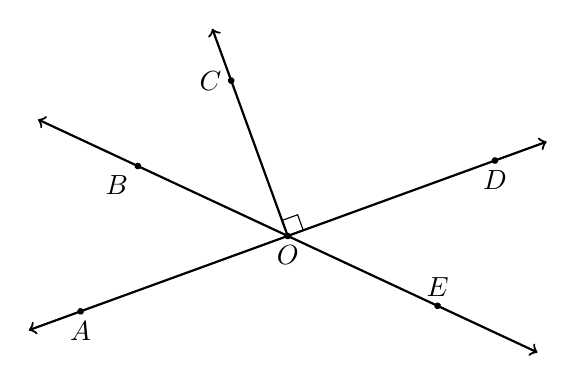
\begin{tikzpicture}[scale=0.7, rotate=20]
      \draw [<->, thick] (-45:5)--(0,0)--(135:5);
      \draw [<->, thick] (-5,0)--(5,0);
      \draw [->, thick] (0,0)--(0,4);
      \draw (0,0)++(0.3,0)--++(0,0.3)--+(-0.3,0);
      \draw [fill] (135:3) circle [radius=0.05] node[below left]{$B$};
      \draw [fill] (-4,0) circle [radius=0.05] node[below]{$A$}; 
      \draw [fill] (0,0) circle [radius=0.05] node[below]{$O$};
      \draw [fill] (0,3) circle [radius=0.05] node[left]{$C$};
      \draw [fill] (4,0) circle [radius=0.05] node[below]{$D$};
      \draw [fill] (-45:3) circle [radius=0.05] node[above]{$E$};
      \end{tikzpicture}
  \end{center}
\end{multicols}
Copy the correct equation and solve for $x$. Check your answer. \vspace{6cm}

\item Given the rectangle $ABCD$, shown below, with $AB=11$ and $AD=5$. Find its area.
    \begin{flushright}
    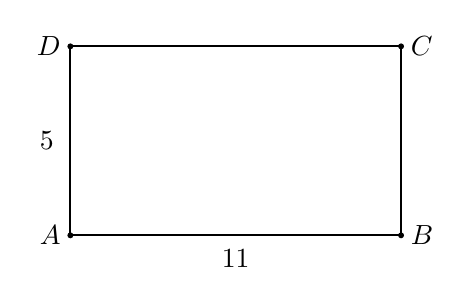
\begin{tikzpicture}[scale=0.6]
      \draw [-, thick] (0,0)--(7,0)--(7,4)--(0,4)--cycle;
      \draw [fill] (0,0) circle [radius=0.05] node[left]{$A$};
      \draw [fill] (7,0) circle [radius=0.05] node[right]{$B$};
      \draw [fill] (7,4) circle [radius=0.05] node[right]{$C$};
      \draw [fill] (0,4) circle [radius=0.05] node[left]{$D$};
      \node at (-0.5, 2){5};
      \node at (3.5, -0.5){11};
    \end{tikzpicture}
    \end{flushright}

\item Find the area of the rectangle $MATH$ shown below, with $MA=4.7$ and $MH=1.9$.
    \begin{flushleft}
    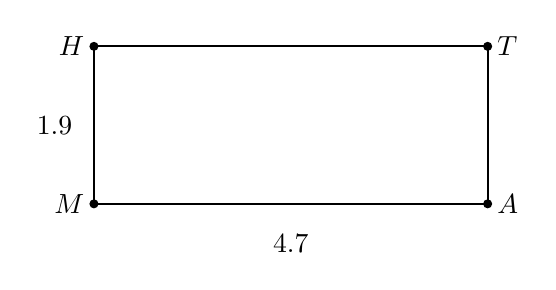
\begin{tikzpicture}
      \draw [-, thick] (0,0)--(5,0)--(5,2)--(0,2)--cycle;
      \draw [fill] (0,0) circle [radius=0.05] node[left]{$M$};
      \draw [fill] (5,0) circle [radius=0.05] node[right]{$A$};
      \draw [fill] (5,2) circle [radius=0.05] node[right]{$T$};
      \draw [fill] (0,2) circle [radius=0.05] node[left]{$H$};
      \node at (-0.5, 1){1.9};
      \node at (2.5, -0.5){4.7};
    \end{tikzpicture}
    \end{flushleft}

\newpage

\item Find the combined area of the shape shown below, a rectangle and a square. The grid is in centimeters.
    \begin{flushleft}
      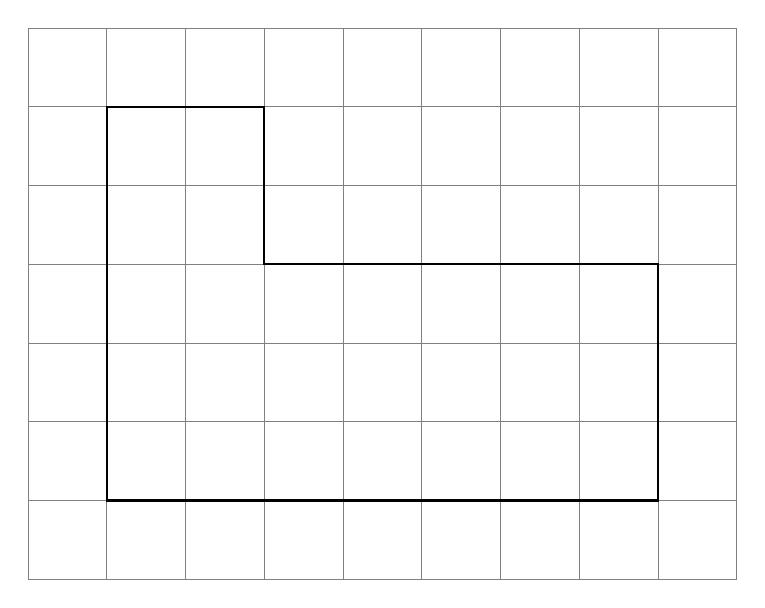
\begin{tikzpicture}[scale=1]
        \draw [help lines] (-4,-4) grid (5,3);
        %\draw [thick, ->] (-2.2,0) -- (10.4,0) node [below right] {$x$};
        %\draw [thick, ->] (0,-2.2)--(0,10.4) node [left] {$y$};
        %\draw (0,0) circle [radius=3] node[below]{$C$};
        %\draw [fill] (0,0) circle [radius=0.05];
        \draw [thick, -] (-3,-3)--(4,-3)--(4,0)--(-1,0)--(-1,2)--(-3,2)--cycle;
      \end{tikzpicture}
    \end{flushleft} \vspace{0.5cm} 

\item The compound shape shown below is composed of a square with side length 5 cm and a triangle with base 2 cm. Find the total area of the combined shape.
    \vspace{1cm} 
    \begin{flushleft}
    \begin{tikzpicture}
      \draw [-, thick] (0,0)--(7,0)--(5,5)--(0,5)--cycle;
      \draw [dashed] (5,0)--(5,5);
      %\draw [fill] (0,0) circle [radius=0.05] node[left]{$A$};
      %\draw [fill] (7,0) circle [radius=0.05] node[right]{$B$};
      %\draw [fill] (7,2) circle [radius=0.05] node[right]{$C$};
      %\draw [fill] (0,2) circle [radius=0.05] node[left]{$D$};
      \node at (6, -0.5){2};
      \node at (2.5, -0.5){5};
      \node at (-0.5, 2.5){5};
    \end{tikzpicture}
    \end{flushleft} \vspace{1cm}
\item Repeat the calculation for the figure above using the trapezoid area formula.

\end{enumerate}
\end{document}